\section{量子物理}
\sourceproblem{选择1}{67}{73}
\problemtext 判断绝对黑体的吸收、反射与发射性质。
\workings 理想黑体吸收全部入射电磁辐射，不反射也不透射，选D。
\crosscheck 黑体在非零温度可发射热辐射，不是不能发射的物体。
\sourceproblem{选择2}{67}{73}
\problemtext 同一金属入射光由400 nm变为300 nm，求遏止电压变化。
\workings $e\Delta U_s=hc(1/\lambda_2-1/\lambda_1)$，取题给常数得 $\Delta U_s\approx1.036$ V，选C。
\crosscheck 逸出功抵消；两次均须发生光电效应。
\sourceproblem{选择3}{67}{73}
\problemtext 钨的红限230 nm，180 nm光照射时求最大光电子动能。
\workings $K_{\max}=hc(1/180-1/230)$，此处波长用nm并换算为m；结果约1.50 eV，选C。
\crosscheck 入射波长小于红限，动能非负。
\sourceproblem{选择4}{67}{73}
\problemtext 真空中波长 $\lambda$ 的光子的能量和动量大小。
\workings $E=h\nu=hc/\lambda,\ p=E/c=h/\lambda$，选A。
\crosscheck 光子静质量为零但能量与动量不为零。
\sourceproblem{选择5}{67}{73}
\problemtext 康普顿散射中何种散射角使散射光频率下降最多。
\workings 静止自由电子模型中 $\Delta\lambda=h(1-\cos\phi)/(m_ec)$，在 $\phi=\pi$ 最大，频率最小，选A。
\crosscheck 波长增大与频率下降对应；不把散射角与反冲电子角混淆。
\sourceproblem{选择6}{67}{73}
\problemtext 同一金属入射频率由 $\nu$ 变为 $2\nu$，原最大动能 $E_k$，求新最大动能。
\workings $E_k=h\nu-W$，故 $E'_k=2h\nu-W=h\nu+E_k$，选D。
\crosscheck 逸出功不随光频率改变。
\sourceproblem{选择7}{67}{73}
\problemtext 氢基态电离能13.6 eV，某激发态电离能0.544 eV，求主量子数。
\workings 玻尔模型 $13.6/n^2=0.544$，得 $n=5$，选B。
\crosscheck 束缚态能量为负，电离能为其绝对值。
\sourceproblem{选择8}{67}{73}
\problemtext 基态氢原子至少吸收多少能量，才能在退激时发射可见谱线（选项续PDF74）。
\workings 可见巴耳末系最低跃迁为 $3\to2$，故至少激发到 $n=3$。$\Delta E=13.6(1-1/9)=12.0889$ eV，选D。
\crosscheck $2\to1$ 为紫外，不满足可见光条件；激发到3后存在发射可见光的可能，并非每次都发出。
\sourceproblem{选择9}{68}{74}
\problemtext 氢原子处于 $n=3$ 时的电离能。
\workings $E_{\rm ion}=13.6/9\approx1.51$ eV，选D。
\crosscheck 不用基态至第三能级的激发能12.09 eV代替电离能。
\sourceproblem{选择10}{68}{74}
\problemtext 从给定光子能量中选择能被 $n=2$ 氢原子吸收者。
\workings $2\to3$ 能量差 $13.6(1/4-1/9)=1.8889$ eV，选B。其余选项不匹配允许的离散能级差且低于电离阈值3.4 eV。
\crosscheck 采用理想离散能级、忽略谱线展宽与精细结构的模型。
\sourceproblem{填空1}{68}{74}
\problemtext 金属红限 $\lambda_0$，入射波长 $\lambda<\lambda_0$，求逸出电子动量。
\workings 最大动能 $K_{\max}=hc(1/\lambda-1/\lambda_0)$，非相对论最大动量 $p_{\max}=\sqrt{2m_ehc(1/\lambda-1/\lambda_0)}$。若需相对论精确式则 $p_{\max}c=\sqrt{K_{\max}(K_{\max}+2m_ec^2)}$。
\crosscheck 实际逸出电子有能量分布，题给数据只能确定最大动量，而非每个电子的动量。
\sourceproblem{填空2}{68}{74}
\problemtext 0.5 MeV光子发生康普顿散射，反冲电子能量0.1 MeV，求波长增量与入射波长比。
\workings 将题给电子能量理解为增加的动能，散射光子能量0.4 MeV。$\Delta\lambda/\lambda_0=0.5/0.4-1=1/4$。
\crosscheck 若0.1 MeV被理解为电子总能量则低于电子静能，不可能；教材意指反冲动能。以初始静止自由电子模型检验，$1-\cos\phi=m_ec^2(1/E'-1/E)\approx0.2555$，故 $\phi\approx41.9^\circ$，符合康普顿散射的运动学范围。
\sourceproblem{填空3}{68}{74}
\problemtext 大量处于 $n=3$ 的氢原子退激，求可能的不同波长数。
\workings 三个能级间下跃迁为 $3\to2,3\to1,2\to1$，共3种。
\crosscheck 大量原子可走不同级联路径，单个原子一次退激不一定发出三种光。
\sourceproblem{填空4}{68}{74}
\problemtext 玻尔模型中第四轨道电子动能与基态动能比。
\workings 库仑圆轨道 $K_n=13.6/n^2$ eV，故 $K_4/K_1=1/16$。
\crosscheck 动能为正而总能量为负。
\sourceproblem{填空5}{68}{74}
\problemtext 玻尔模型第五轨道与第一激发态的角动量比。
\workings $L_n=n\hbar$，第一激发态 $n=2$，故比值5/2。
\crosscheck 现代量子力学轨道角动量由 $l$ 决定；此题指定玻尔模型。
\sourceproblem{填空6}{68}{74}
\problemtext 玻尔模型第一与第三轨道速率比。
\workings 由 $m_ev_nr_n=n\hbar$ 且 $r_n=n^2a_0$，得 $v_n\propto1/n$，故 $v_1/v_3=3$。
\crosscheck 不将半径平方比误用为速度比。
\sourceproblem{计算1}{69}{75}
\problemtext 光电效应中入射波长500 nm降至400 nm，求遏止电压变化。
\workings $e\Delta U_s=hc(1/400\,\mathrm{nm}-1/500\,\mathrm{nm})$。取题给 $h=6.63\times10^{-34}$、$e=1.60\times10^{-19}$，得 $\Delta U_s=0.62156$ V，增大。
\crosscheck 两次均可产生光电子，逸出功相同；电压变化为正。
\sourceproblem{计算2}{69}{75}
\problemtext 500 nm光照射金属，光电子最大动能0.7 eV，求红限波长。
\workings $hc/\lambda_0=hc/(500\,\mathrm{nm})-0.7\,\mathrm{eV}$。用题给常数及 $c=3\times10^8$ m/s，得逸出功1.78625 eV，$\lambda_0\approx696$ nm。
\crosscheck 红限长于入射波长，回代能量差为0.7 eV。
\sourceproblem{计算3}{70}{76}
\problemtext 基态氢吸收12.09 eV光子后，求玻尔轨道半径增加倍数。
\workings $13.6(1-1/n^2)\approx12.09$ eV，故 $n=3$，$r_3/r_1=9$。末半径为原来的9倍，净增量为原半径的8倍。
\crosscheck 原题能量取两位小数，匹配离散能级需按舍入精度理解；区分增加到与净增加。
\sourceproblem{计算4}{70}{76}
\problemtext 基态氢吸收12.75 eV，求激发能级、所有可能退激谱线及能级图。
\workings $13.6(1-1/n^2)=12.75$，得 $n=4$。在玻尔能级近似下 $E_n=-13.6/n^2$ eV，六种向下跃迁的光子能量分别为 $4\to3:0.6611$、$4\to2:2.55$、$4\to1:12.75$、$3\to2:1.8889$、$3\to1:12.0889$、$2\to1:10.20$ eV，取 $hc\simeq1239.84\,\mathrm{eV\,nm}$，按上述顺序，波长约为 $1875.4,\ 486.2,\ 97.24,\ 656.4,\ 102.56,\ 121.55\,\mathrm{nm}$。这些数值采用题给13.6 eV的能级近似，不是精密实验谱线。
\begin{center}
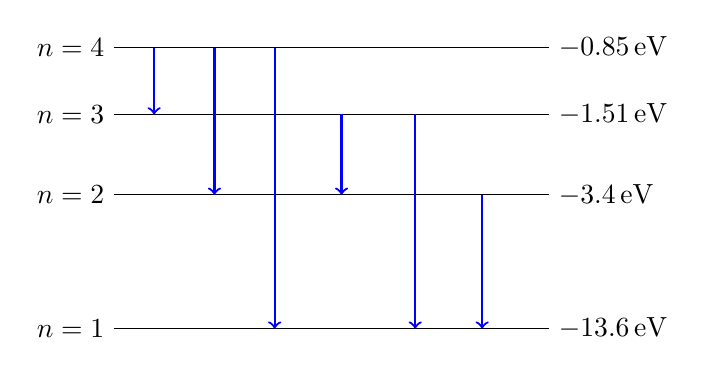
\begin{tikzpicture}[scale=.85]
\foreach \y/\n/\en in {0/1/-13.6,2/2/-3.4,3.2/3/-1.51,4.2/4/-0.85}{
\draw (0,\y)--(6.5,\y); \node[left] at (0,\y) {$n=\n$}; \node[right] at (6.5,\y) {$\en\,\mathrm{eV}$};}
\draw[->,blue,thick] (.6,4.2)--(.6,3.2);
\draw[->,blue,thick] (1.5,4.2)--(1.5,2);
\draw[->,blue,thick] (2.4,4.2)--(2.4,0);
\draw[->,blue,thick] (3.4,3.2)--(3.4,2);
\draw[->,blue,thick] (4.5,3.2)--(4.5,0);
\draw[->,blue,thick] (5.5,2)--(5.5,0);
\end{tikzpicture}
\end{center}
\crosscheck 图为定性能级图，间距非线性比例；六种为大量原子、仅考虑主量子数的可能谱线，实际跃迁还受选择定则约束。
